%!TEX program = lualatex
% Arquivo: Template_Estat_Texto.tex

\documentclass[a4paper,12pt]{article}

% =========================================================
% Idioma e tipografia (LuaLaTeX)
% =========================================================
\usepackage[portuguese]{babel}
\usepackage{fontspec}
\setmainfont{Latin Modern Roman}

% =========================================================
% Layout
% =========================================================
\usepackage[top=3cm,bottom=2.5cm,left=3cm,right=2.5cm]{geometry}
\usepackage{setspace}
\onehalfspacing
\usepackage{indentfirst}
\setlength{\parindent}{1.25cm}

% =========================================================
% Matemática (align*, etc.)
% =========================================================
\usepackage{amsmath}
\usepackage{amssymb}
\usepackage{siunitx}

% =========================================================
% Tabelas, listas, figuras
% =========================================================
\usepackage{booktabs}
\usepackage{array}
\usepackage{enumitem}
\setlist[itemize]{noitemsep,topsep=3pt}
\setlist[enumerate]{noitemsep,topsep=3pt}

\usepackage{graphicx}
\usepackage{float}
\usepackage{pdflscape}
\graphicspath{{./}{./imagens/}{./figuras/}}

% =========================================================
% Links
% =========================================================
\usepackage{hyperref}
\usepackage{xurl}
\hypersetup{
  colorlinks=true,
  linkcolor=black,
  urlcolor=blue,
  citecolor=black,
  pdfauthor={},
  pdftitle={}
}

% =========================================================
% Texto de preenchimento (lorem)
% =========================================================
\usepackage{lipsum}

% =========================================================
% Dados da capa
% =========================================================
\newcommand{\Instituicao}{Universidade / Instituição}
\newcommand{\Curso}{Oceanodrafia -- Estatística II}
\newcommand{\Professor}{Professor: Maria Elvira\\ melvira@ime.uerj.br}
\newcommand{\Aluno}{Aluno: José Mauro Xavier Elsas}
\newcommand{\Cidade}{Rio de Janeiro}
\newcommand{\Ano}{2026}

\title{\textbf{Título do Documento}}
\author{\Aluno}
\date{\Cidade --- \Ano}

\begin{document}

% =========================================================
% Capa (página de rosto)
% =========================================================
\begin{titlepage}
\centering
{\large \Instituicao \par}
\vspace{0.5cm}
{\large \Curso \par}
\vspace{1.0cm}

{\LARGE \textbf{Análise exploratória de dados} \par}
\vspace{0.6cm}
{\Large Produção de 40 Pessegueiros \par}

\begin{figure}[H]
  \centering
  
\includegraphics[width=.3\linewidth]{./uerj.jpg}
\end{figure}

\vfill



\begin{flushright}
\Aluno\\
\Professor
\end{flushright}

\vspace{1.0cm}
{\Cidade --- \Ano \par}
\end{titlepage}

% =========================================================
% Sumário
% =========================================================
\tableofcontents
\newpage

% =========================================================
% Corpo do texto (exemplos)
% =========================================================
\section{Exercício}



\begin{table}[H]
  \centering
\begin{tabular}{ll|ll}
\toprule
i&$x_i$&i&$x_i$\\
\midrule
1 & 11,1 & 21 & 21,0 \\
2 & 4,4 & 22 & 18,5 \\
3 & 10,7 & 23 & 12,2 \\
4 & 23,5 & 24 & 19,1 \\
5 & 26,2 & 25 & 3,2 \\
6 & 12,5 & 26 & 16,4 \\
7 & 6,1 & 27 & 16,4 \\
8 & 15,8 & 28 & 12,6 \\
9 & 14,8 & 29 & 7,4 \\
10 & 3,5 & 30 & 8,1 \\
11 & 32,4 & 31 & 11,2 \\
12 & 27,5 & 32 & 15,1 \\
13 & 25,0 & 33 & 4,7 \\
14 & 22,6 & 34 & 9,2 \\
15 & 16,2 & 35 & 12,9 \\
16 & 7,8 & 36 & 22,3 \\
17 & 32,8 & 37 & 6,0 \\
18 & 18,2 & 38 & 13,7 \\
19 & 16,0 & 39 & 10,0 \\
20 & 14,5 & 40 & 19,1\\
\bottomrule
\end{tabular}
  \caption{Produção de 40 Pessegueiros}
\label{tab:pessegueiro}
\end{table}

\section{Resultados descritivos}

\begin{table}[H]
  \centering
\begin{tabular}{ll}
  \toprule
Medida & Valor \\
Média & 15,02 \\
Mediana & 14,65 \\
Variância & 57,03 \\
Desvio padrão & 7,55 \\
N & 40 \\
Valor máximo & 32,8 \\
Valor mínimo & 3,2\\
\bottomrule
\end{tabular}
\caption{}
\label{tab:pesse_desc}
\end{table}

\section{Amplitude da série}

A amplitude da série é dada pela diferença entre o valor máximo e o valor mínimo observados:

\[
A = 32,8 - 3,2 = 29,6
\]

\subsection{Número de classes}

Considerando:

\[
N = 40
\]

Podem ser utilizadas as seguintes expressões para estimar o número de classes:

\[
\begin{cases}
\sqrt{40} \approx 6,32, \\
1 + 3,3\log 40 \approx 6,28
\end{cases}
\]

Adotando 6 classes, a amplitude de cada classe é:

\[
A_c = \frac{29,6}{6} \approx 4,93 \approx 5
\]

A Tabela \ref{tab:freq_pessegueiros} apresenta a distribuição de frequências da produção, incluindo frequências absoluta, relativa e acumulada.

\begin{table}[H]
  \centering
    \begin{tabular}{lrrr}
      \toprule
      Produção & $f_a$ & $f_i$ (\%) & $f_{ac}$ (\%)\\
      \midrule
      3 $\vdash$ 8    & 8   & 20,0  & 20,0   \\
      8 $\vdash$ 13   & 10  & 25,0  & 45,0  \\
      13 $\vdash$ 18  & 9   & 22,5  & 67,5  \\
      18 $\vdash$ 23  & 7   & 17,5  & 85,0  \\
      23 $\vdash$ 28  & 4   & 10,0  & 95,0 \\
      28 $\vdash$ 33  & 2   & 5,0   & 100,0 \\
      \midrule
      $\sum f_a$ & 40 & 100,0 & \\
      \bottomrule
    \end{tabular}
\caption{Distribuição de frequências da produção de 40 pessegueiros.}
\label{tab:freq_pessegueiros}
\end{table}

\subsection{Histograma}

\begin{figure}[H]
  \centering
    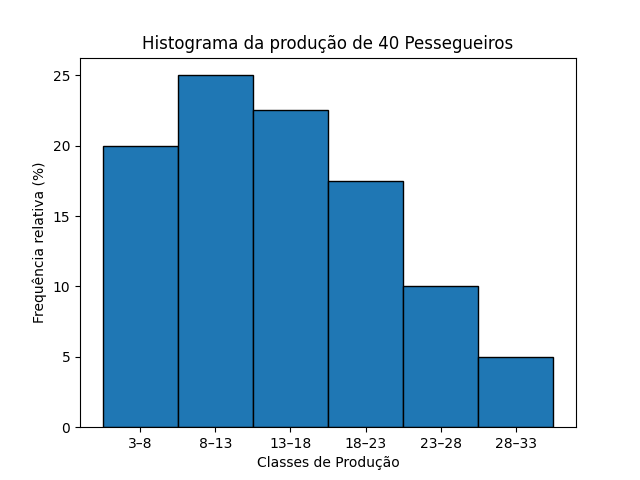
\includegraphics[width=0.9\linewidth]{./Figs/Histo_pesseg.png}
  \caption{Histograma da produção de 40 pessegueiros.}
\end{figure}

\subsection{Frequências acumuladas}

\begin{figure}[H]
  \centering
    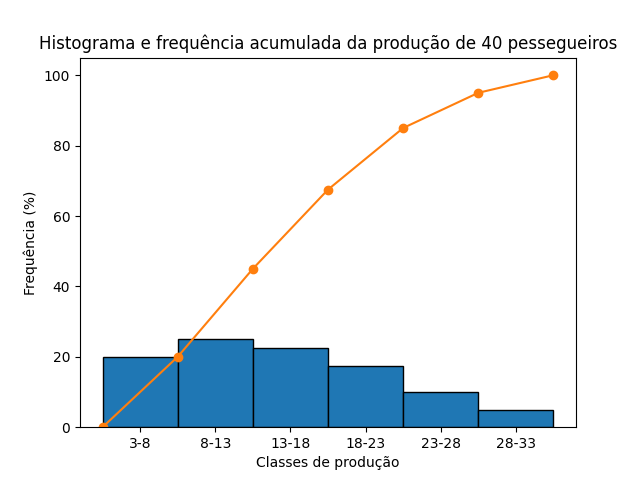
\includegraphics[width=0.9\linewidth]{./Figs/ogiva_pesseg.png}
  \caption{Ogiva das frequências acumuladas das alturas dos alunos.}
\end{figure}
\end{document}